%%
%% (
%%  )\ )                             (
%%  (()/(   (            (             )\  )   (
%%   /(_))  ))\   (       ))\  (   (   (()/(   ))\
%%   (_))  /((_)  )\  )  /((_) )\  )\   ((_))/((_)
%%   | _ \(_))(  _(_/( (_) )  ((_)((_)  _| |(_))
%%   |   /| || || ' \))/ -_)/ _|/ _ \/ _` |/ -_)
%%   |_|_\ \_,_||_||_| \___|\__|\___/\__,_|\___|
%%

\documentclass{article}
\usepackage[utf8x]{inputenc}
\usepackage{amsmath}
%\usepackage{slashbox}
\usepackage{amsfonts}
\usepackage{amssymb}
\usepackage{graphicx} % Paquete para incluir imágenes en el documento LaTeX
\usepackage{hyperref}
\hypersetup{
  colorlinks=true,
  linkcolor=blue,
  filecolor=magenta,
  urlcolor=cyan,
}
\urlstyle{same}
\usepackage{varwidth}

\newcommand\tab[1][1cm]{\hspace*{#1}}

\usepackage{multirow}

\usepackage[a4paper,rmargin=1.5cm,lmargin=1.5cm,top=1.5cm,bottom=1.5cm]{geometry}

\usepackage{pdfpages}

\usepackage{xcolor}
\usepackage{minted}
\setminted[cpp]{frame=lines, framesep=2mm, baselinestretch=1.2, rulecolor=\color{black!80},
                bgcolor=DarkGray,fontsize=\normalsize}
\usemintedstyle[cpp]{monokai}
\setminted[python]{frame=lines, framesep=2mm, baselinestretch=1.2, rulecolor=\color{black!80}, bgcolor=DarkGray}
\usemintedstyle[python]{monokai}
\setminted[java]{frame=lines, framesep=2mm, baselinestretch=1.2, rulecolor=\color{black!80}, bgcolor=DarkGray}
\usemintedstyle[java]{monokai}
\setminted[javascript]{frame=lines, framesep=2mm, baselinestretch=1.2, rulecolor=\color{black!80}, bgcolor=DarkGray}
\usemintedstyle[javascript]{monokai}
\setminted[php]{frame=lines, framesep=2mm, baselinestretch=1.2, rulecolor=\color{black!30}, bgcolor=LightGray}
\setminted[html]{frame=lines, framesep=2mm, baselinestretch=1.2, rulecolor=\color{black!30}, bgcolor=LightGray}
\setminted[bash]{baselinestretch=1.2,rulecolor=\color{black!30},fontsize=\footnotesize,bgcolor=LightGray}
\definecolor{LightGray}{gray}{0.98}
\definecolor{DarkGray}{gray}{0.1}
\definecolor{MidGray}{gray}{0.8}
\definecolor{codegreen}{rgb}{0,0.6,0}
\definecolor{codegray}{rgb}{0.5,0.5,0.5}
\definecolor{codepurple}{rgb}{0.58,0,0.82}
\definecolor{backcolour}{rgb}{0.95,0.95,0.92}

\setlength{\parindent}{0px}  % Setea la indentacion de la primera linea de cada parrafo a cero pixeles.


\title{Introducción a JavaSE}
\author{@RuneCode}

\begin{document}
%% Portada
\includepdf{./portada/portada.pdf}

%% Clase 1
\section{¿Qué es Java?}%
Java es un lenguaje de programación en alto nivel (aunque no tan alto como
Python o JavaScript) que nos ayuda a construir aplicaciones para diferentes
dispositivos y sistemas operativos.\\

Fue creado en 1991 por James Gosling mientras trabajaba en Sun Microsystems,
una empresa que luego fue adquirida por Oracle. Esto significa que Java tiene
muy buen mantenimiento, pero también algunos cambios con los que no todos
estaremos de acuerdo.\\

Java tiene dos categorías: Standard Edition para construir aplicaciones de
escritorio o consola y Enterprise Edition para que las empresas trabajen
aplicaciones web de última generación.\\

En este curso aprenderemos los fundamentos de Java Standard Edition: la
sintaxis del lenguaje, declarar variables, trabajar con funciones, ciclos y
condicionales, lógica de programación, algoritmos y muchas otras cosas.\\

Pero no te preocupes, Java sigue la filosofía de Write Once, Run Anywhere
(WORA), por lo que todo lo que aprendas en este curso lo podrás aplicar también
con Java EE.\\


%% Clase 2
\section{Versiones de Java y JDK}%
El JDK o Java Development Kit se compone de los siguientes elementos:
\begin{itemize}
  \item \textbf{Java Runtime Enviroment (JRE)}: La máquina virtual de Java, lo
    que nos permite que al escribir el mismo código funciones igual en todos
    los dispositivos y sistemas operativos.
  \item \textbf{Compilador de Java}: El encargado de traducir nuestro código en
    Java a un lenguaje que puede entender e interpretar nuestra máquina
    virtual.
  \item \textbf{APIs de desarrollo}: Una base de código listo para ayudarnos a
    desarrollar.
\end{itemize}

Las APIs de desarrollo con Java han evolucionado con el tiempo, por lo que
existen diferentes versiones de java que puedes utilizar. La versión que más
elevo la popularidad y las ofertas de trabajo con Java fue Java SE 6.\\

En Java SE 9 anunciaron que las actualizaciones ocurririan cada 6 meses, pero
las versiones LTS (Long Time Support) tendrán mantenimiento por 3 años, así que
las actualizaciones son necesarias, pero no urgentes.\\

En este curso vamos a trabajar con la versión Java SE 11 LTS, la primera
versión de Java con licencia. Solo podremos usarlo gratis cuando trabajemos en
ambientes de desarrollo y testing. De otra forma, debemos pagar 2.5 USD al mes
por usarlo de escritorio y 25 USD por procesador para aplicaciones de
servidor.\\

Afortunadamente, OpenJDK es una versión gratis y open source de usar Java SE
Platform Edition.\\

%% Clase 3
\section{Las herramientas más usadas de Java}%
Java 8 (LTS) es la versión más usada de Java hasta inicios del 2019, pero solo
tendrá soporte hasta diciembre del 2020, luego de esta fecha tendremos que
pagar una licencia para continuar con su soporte.\\

Java 10 introdujo algunos cambios en la forma de declarar variables, así que en
este curso vamos a trabajar con las versiones 8 y 11 de Java.\\

La herramienta más usada para construir proyectos web con Java es Maven, pero
también existen otras alternativas como Grandle. También existen frameworks
como Spring para trabajar con Java EE y ORMs como Hiberante para trabajar con
bases de datos.\\

Los IDEs son entornos de desarrollo integrados, herramientas (aplicaciones,
seguramente de escritorio) que nos ayudan a escribir nuestro código con
editores, compiladores, depuradores y constructores de interfaces gráficas,
todo en un mismo lugar.\\

El IDE recomendado por Oracle es NetBeans, pero también están Eclipse e InteliJ
IDEA, este último es el que más fuerza ha tomado gracias a Kotlin. Las tres
herramientas son gratuitas, pero IntelliJ IDEA también tiene una versión de
pago.\\


%% Clase 4
% \section{Creando un Entorno de Desarrollo en Java en Windows}%

%% Clase 5
% \section{Creando un Entorno de Desarrollo en Java en Mac}%

%% Clase 6
\section{Creando un Entorno de Desarrollo en Java en Linux}%
\textbf{Instalar Openjdk Java}\\
Para eso usaremos nuestro gestor de paquerería \textbf{apt}, con el siguiente
comando:\\

\begin{minted}{bash}
  sudo apt install default-jre
\end{minted}

\begin{figure}[h!]
    \centering
      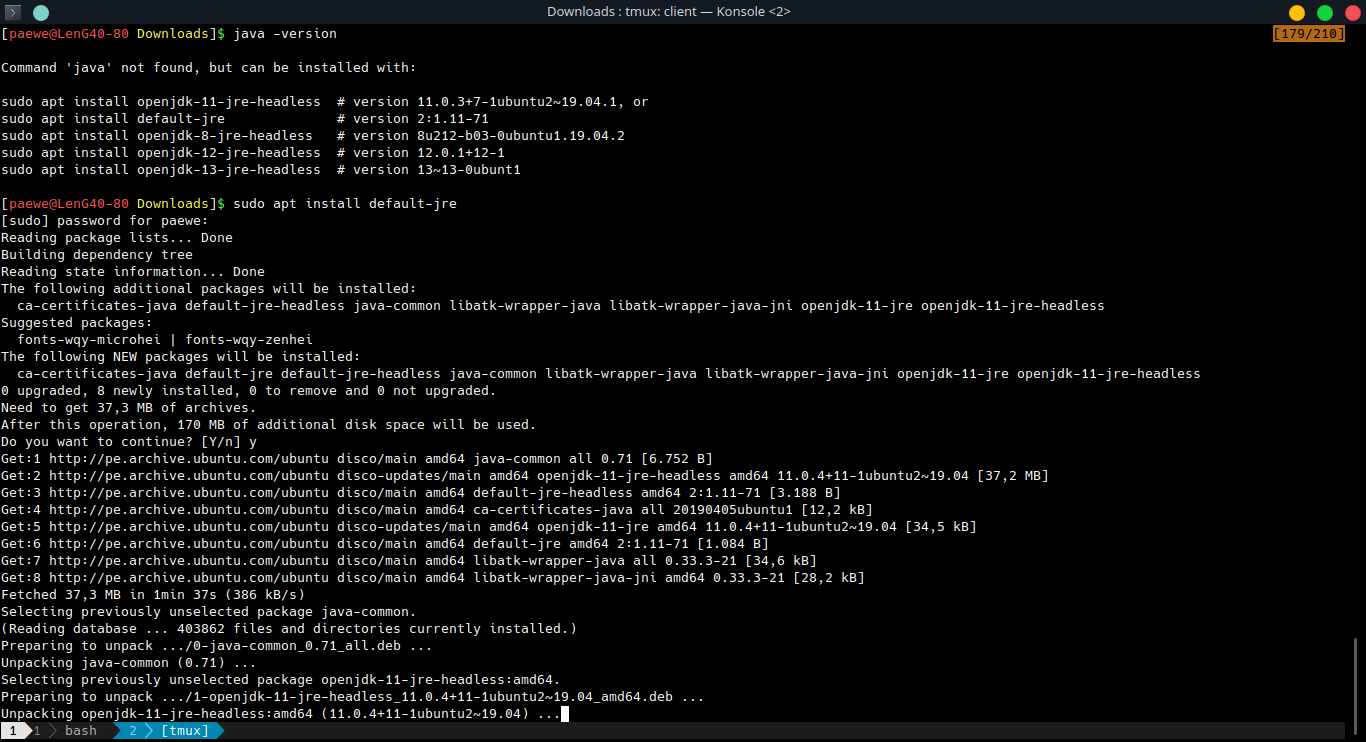
\includegraphics[scale=0.5]{./Pictures/002_openjdk_default.png}
\end{figure}

Con esto se instala la versión Openjdk 11 que es por defecto para Ubuntu 18.04.\\

Se puee verificar la version de Java usada por el sistema con el siguiente comando:
\begin{minted}{bash}
  java -version
\end{minted}

\begin{figure}[h!]
    \centering
      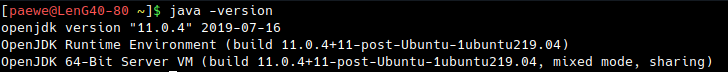
\includegraphics[scale=0.75]{./Pictures/004_javaversion1.png}
\end{figure}

Luego vamos a instalar la versión Openjdk 8 con el siguiente comando:

\begin{minted}{bash}
  sudo apt install openjdk-8-demo openjdk-8-doc openjdk-8-jdk openjdk-8-source
\end{minted}

\begin{figure}[h!]
    \centering
      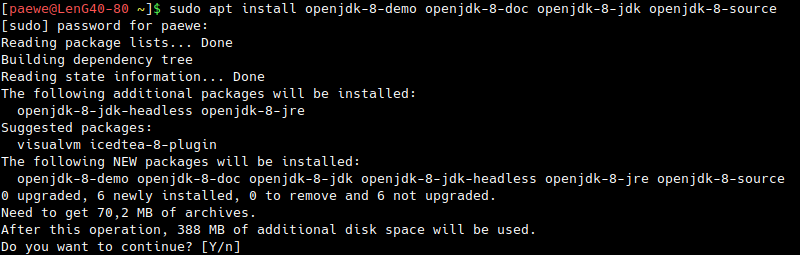
\includegraphics[scale=0.75]{./Pictures/030_install_openjdk_ijidea.png}
\end{figure}

\newpage

\textbf{Instalar Oracle Java SE 8}\\
Para esto vamos al siguiente
\href{https://www.oracle.com/technetwork/java/javase/downloads/index.html}{enlace}.\\

Luego escogemos la versión de Java SE 8u221 y se elige como se muestra en la
siguiente imágen:\\

\begin{figure}[h!]
    \centering
      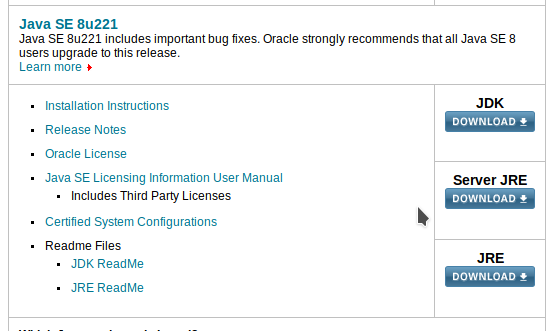
\includegraphics[scale=0.75]{./Pictures/001_javaSEOracle.png}
\end{figure}

Luego descomprimimos usando \textbf{tar} y copiamos la carpeta en la ruta
\textbf{/usr/jvm}. Después de esto se da la instalación usando el siguiente
comando:\\

\begin{minted}{bash}
  sudo update-alternatives --install /usr/bin/java java /usr/jvm/jdk1.8.0_221/bin/java 1
\end{minted}


\begin{figure}[h!]
    \centering
      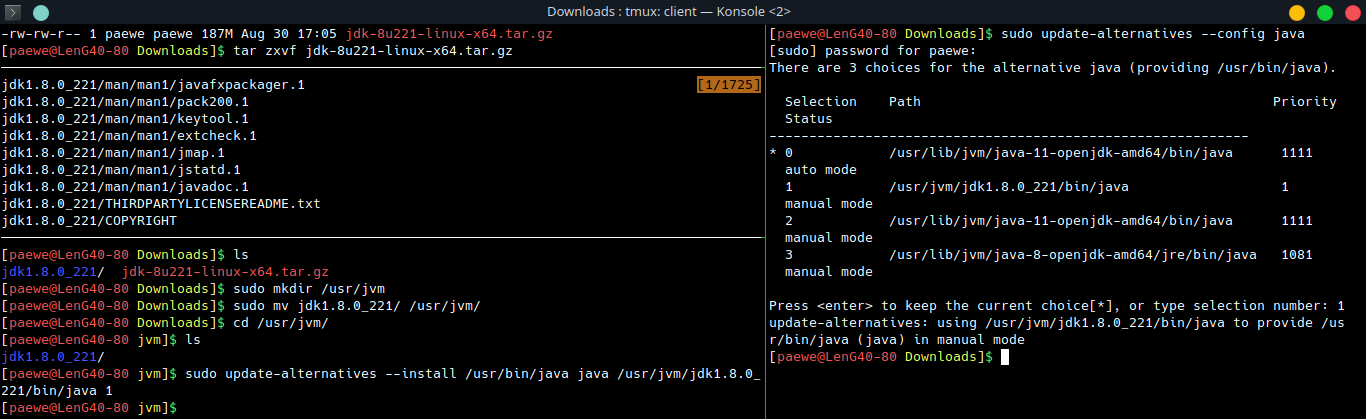
\includegraphics[scale=0.5]{./Pictures/005_oraclejavaselect.png}
\end{figure}


Después comprobamos la versión de java usada por el sistema.\\

\begin{minted}{bash}
  java -version
\end{minted}

\begin{figure}[h!]
    \centering
      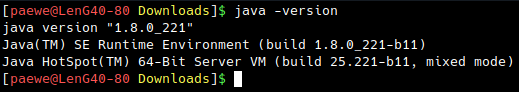
\includegraphics[scale=0.75]{./Pictures/006_javaversion2.png}
\end{figure}

\newpage

Finalmente vamos a configurar nuestra variable de entorno llamada
\textbf{JAVA\_HOME} que muchos programas lo utilizan, por ejemplo Netbeans.
Para eso hacemos lo siguiente:\\

\begin{figure}[h!]
    \centering
      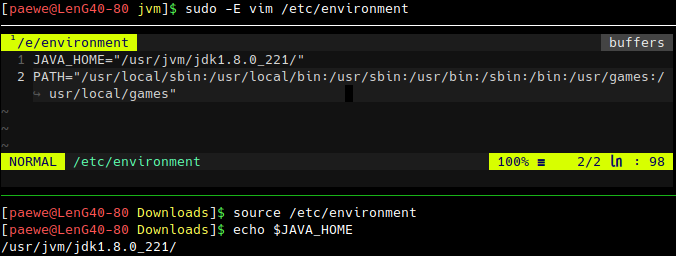
\includegraphics[scale=0.75]{./Pictures/007_java_home.png}
\end{figure}

\textbf{Instalando IntelliJ IDEA en Ubuntu}\\

Para instalar IntelliJ IDEA vamos a usar el gestor \textbf{snap} el cual
podemos instalar primero con el comando:\\

\begin{minted}{bash}
  sudo apt install snap
\end{minted}

Luego nos dirigimos a la página \textbf{snapcraft} donde encontraremos muchos
programas disponibles para instalar usando snap. Visita el siguiente
\href{https://snapcraft.io/intellij-idea-community}{enlace}.\\

Copiamos el comando de instalación, que en ese caso es:

\begin{minted}{bash}
  sudo snap install intellij-idea-community --classic
\end{minted}


%% Clase 7
\section{Escribe tu primer Hola Mundo}%
Los archivos de Java usan la extensión \textbf{.java}. Por lo tanto, para crear
nuestro primer "Hola, mundo" podemos hacerlo desde un archivo
\texttt{HolaMundo.java}.\\

Abrimos IntelliJ IDEA y elegimos la opción  \texttt{Create New Project}.\\

\begin{figure}[h!]
  \centering
  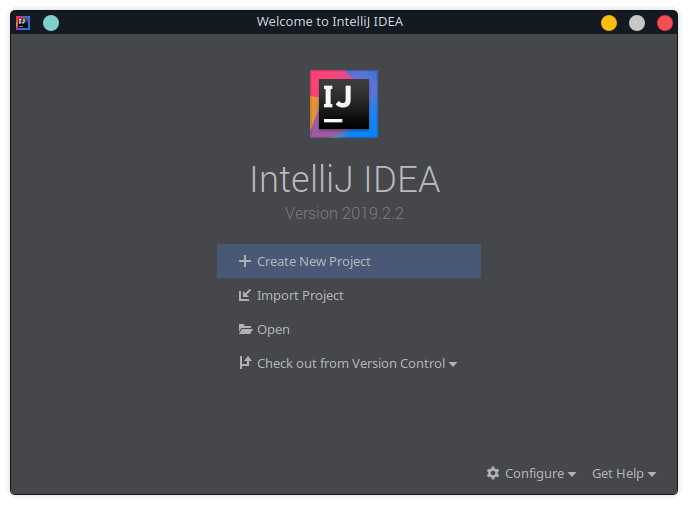
\includegraphics[scale=0.74]{./Pictures/032_crear_proyecto_ij.png}
\end{figure}

Luego escogemos el JDK que en nuestro caso será la version de Java 1.8.0\_222.

\begin{figure}[h!]
  \centering
  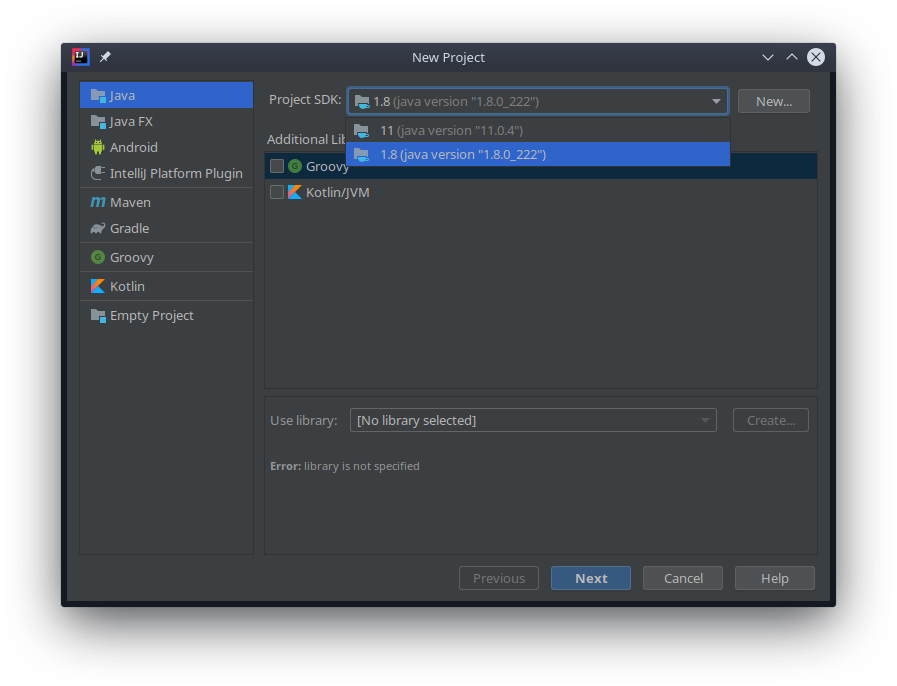
\includegraphics[scale=0.75]{./Pictures/001_escoger_jdk.png}
\end{figure}

Si no aparece esta opción, podremos elegirla desde \textbf{New} y buscamos la ruta:\\

\begin{minted}{bash}
  /usr/lib/jvm/java-1.8.0-openjdk-amd64
\end{minted}

Si prefieres trabajar con la versión JDK 8 de Oracle entonces indicas la ruta
con la que se ha instalado previamente:\\

\begin{minted}{bash}
  /usr/jvm/jdk1.8.0_221
\end{minted}

Para este ejemplo usaremos la versión libre es decir OpenJDK.\\

Después de ingresar el nombre del proyecto habremos terminado con el
precedimiento.\\

\begin{figure}[h!]
  \centering
  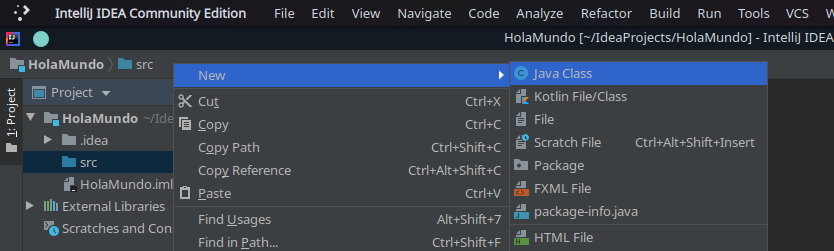
\includegraphics[scale=0.75]{./Pictures/033_crear_clase.png}
\end{figure}

Para crear una clase podemos dar clic derecho en la carpeta \textbf{src} que
figura en el panel de la izquierda y que se despliega del nombre de nuestro
proyecto. Colocamos el nombre de nuestra clase y luego Enter.\\

\begin{figure}[h!]
  \centering
  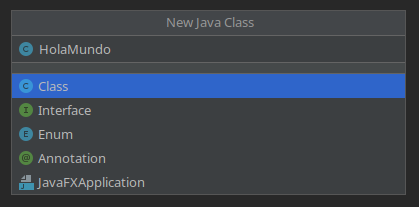
\includegraphics[scale=0.75]{./Pictures/034_new_class.png}
\end{figure}

\textbf{Como se estructura el código en Java}\\

El método \textbf{main} es el punto de entrada de una aplicación en diferentes
lenguajes como Java, Kotlin y C++. Sin este método nuestra aplicación no se
ejecutará y mostrará un error.\\

En Java definimos este método de la siguiente manera:

\begin{minted}{java}
  public static void main (String[] args) {
    // acciones
  }
\end{minted}

Recuerda que Java es un lenguaje POO y por eso el método main se define dentro de una clase.

\begin{minted}{java}
  public class HolaMundo {
    public static void main (String[] args) {
      System.out.println("Hola, mundo!");
    }
  }
\end{minted}

Por lo tanto, este será el código de nuestro \texttt{HolaMundo.java} y podremos
ejecutarlo con\\
\texttt{Clic derecho > Run 'HolaMundo.main()'}:

\begin{figure}[h!]
  \centering
  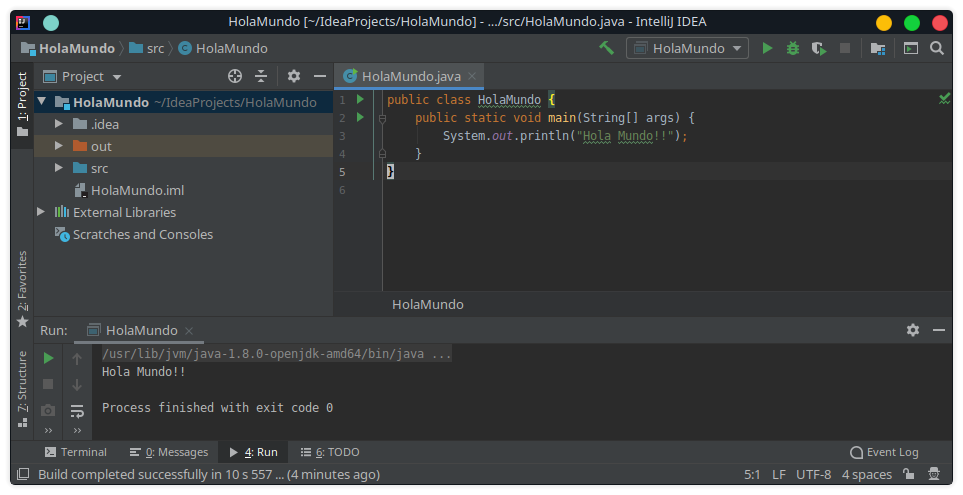
\includegraphics[scale=0.73]{./Pictures/002_IntelliJ_Idea.png}
\end{figure}

Recuerda que nuestro IDE nos proporciona algunos atajos. Por ejemplo, con solo
escribir la palabra \texttt{sout} podremos autocompletar la sentencia
\texttt{System.out.println();} que nos permite imprimir en pantalla.\\

%% Clase 8
\section{Etapas de la programación en Java}%
\begin{enumerate}
  \item Escribir nuestros archivos \texttt{.java}
  \item Compilar, cargar y verificar nuestros archivos con \texttt{javac} (los
    IDEs nos permiten compilar con solo presionar un botón).
  \item Al compilar obtenemos archivos \texttt{.class} con código que nuestras
    computadoras pueden entender (Byte Code).
  \item La JVM (Java Virtual Machine) se encarga de ejecutar el código de forma
    que funcione en cualquier dispositivo o sistema operativo.
\end{enumerate}

Java es un lenguaje compilado e interpretado al mismo tiempo.\\

\begin{figure}[h!]
  \centering
  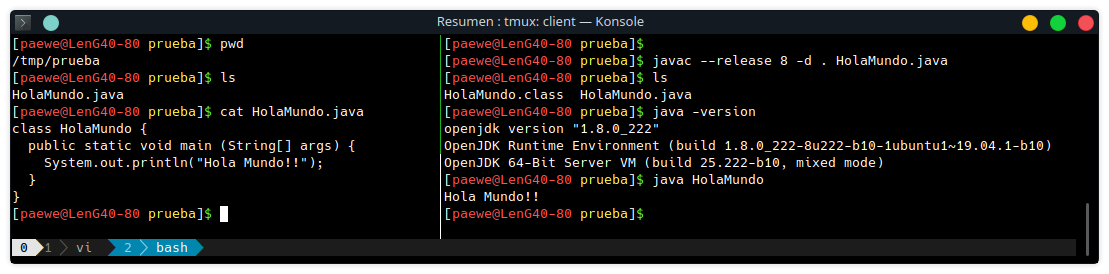
\includegraphics[scale=0.6]{./Pictures/035_compilar_java_terminal.png}
\end{figure}

\textbf{Nota: }Como se ve en la imagen el sistema está usando la version de
Java 8 OpenJDK y para compilar se tiene que usar la opcion \texttt{--release 8}
para que sea compatible con la máquina virtual.\\


\newpage

%% Clase 9
\section{La JShell de Java}%
Sabías que Java tiene una herramienta interactiva en dónde puedes ir probando
segmentos de código en vez de realizar todo el proceso de creación de un
programa en Java. Escribir, compilar y correr.\\

Su nombre es \texttt{jshell} y está disponible desde la versión 9 de Java.\\

Abre tu consola de comandos o terminal, corre el siguiente comando:

\begin{minted}{bash}
  java -version
\end{minted}

\textbf{Ejercicio 1}\\
Investiga cómo cambiar la versión de Java desde tu consola de comandos o
terminal y compártenos en la sección de discusiones los comandos que
ejecutaste.\\

\begin{minted}{bash}
  sudo update-alternatives --config java
\end{minted}

\begin{figure}[h!]
  \centering
  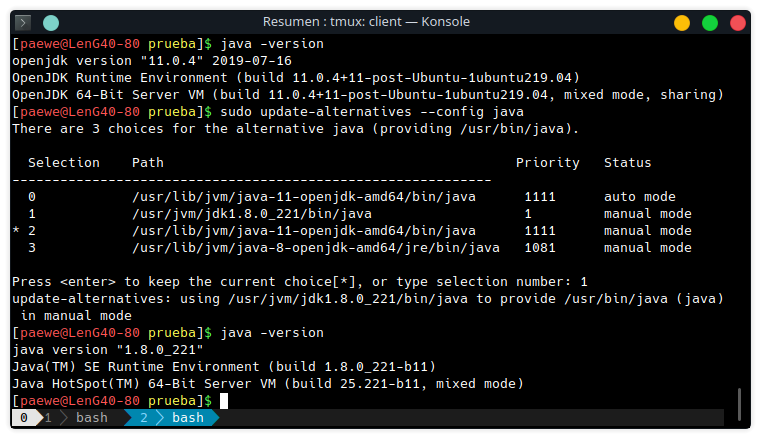
\includegraphics[scale=0.75]{./Pictures/037_update_alternatives.png}
\end{figure}


\textbf{Ejercicio 2}\\
Asegúrate de tener definida una versión superior a la 8.\\
Ahora desde tu terminal escribe el siguiente comando para abrir nuestra \texttt{jshell}

\begin{minted}{bash}
  jshell
\end{minted}

Ahora escribe la línea de código para imprimir un texto (no olvides poner
\textbf{;} y dar enter).

\begin{figure}[h!]
  \centering
  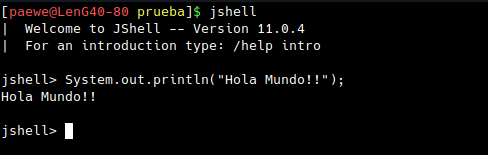
\includegraphics[scale=0.75]{./Pictures/036_jshell.png}
\end{figure}


\newpage

%% Clase 10
\section{Variables en Java}%
Una variable es un espacio de memoria (RAM) que contiene un dato de tipo
numérico, booleano, de texto u otro tipos de datos un poco más complejos.\\

Las variables en Java se componen de un nombre único y un valor que puede
cambiar a lo largo de la ejecución del programa. Al declarar las variables
debemos definir el tipo de dato que vamos a usar y un punto y coma al final:\\

\begin{minted}{java}
  // Variables.java

  public class Variables {
    public static void main (String[] args) {
      // Declarando una variable
      int speed;

      // Asignamos un valor a una variable
      speed = 10;   // Si ya habias declarado la variable
      System.out.println(speed);

      // Declarar una variable y asignarle un valor al mismo tiempo:
      int salary = 1000;

      // Crear una variable de tipo String:
      String employeeName = "Anahí Salgado";
      System.out.println(employeeName);
    }
  }
\end{minted}


%% Clase 11
\section{Actualizando variables}%
Java nos permite actualizar nuestras variables reutilizando los valores que
tenían anteriormente, de esta forma evitamos errores o inconsistencias en
nuestro código:

\begin{minted}{java}
  public class UpdatingVariables {
      public static void main(String[] args) {
          int salary = 1000;

          // bono $200
          salary = salary + 200;
          System.out.println(salary);

          // pension: $50 descuento
          salary = salary - 50;
          System.out.println(salary);

          // 2 horas extra $30 c/u
          // Comida: $45
          salary = salary + (2*30) - 45;
          System.out.println(salary);

          // Actualizando cadenas de texto
          String employeeName = "Anahí Salgado";
          employeeName = employeeName + " Días de la Vega";
          System.out.println(employeeName);

          employeeName = "Irene " + employeeName;
          System.out.println("Tu nombre es: " + employeeName);
      }
  }
\end{minted}

\begin{figure}[h!]
  \centering
  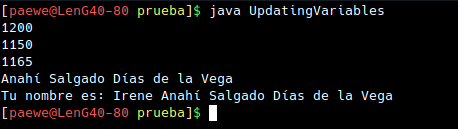
\includegraphics[scale=0.75]{./Pictures/038_updating_variables.png}
\end{figure}


%% Clase 12
\section{Convención de Nombres en Java}%
Una convención de nombres es un patrón que pueden seguir los nombres de las
variables para que el código esté organizado, entendible y sin repetidos.\\

\begin{itemize}
  \item Java es sensible a mayúsculas y minúsculas, este punto es clave al
    seguir una convención.
  \item Las variables siempre deben comenzar con un símbolo de letra, \$ o "\_"
  \item No puedes usar el símbolo - en ninguna parte de la variable.
\end{itemize}

Las variables constantes son variables cuyo valor nunca va a cambiar, por lo
que se deben escribir completamente en mayúsculas y usando el caracter \_


\begin{minted}{java}
  public class NamingJava {
      public static void main(String[] args) {
          int celphone = 33337777;
          int celPhone = 55553333;

          System.out.println(celphone);
          System.out.println(celPhone);

          String $countryName = "Spain";
          String _backgroundColor = "Green";

          String currency$ = "MXN";
          String background_color = "BLUE";

          int POSITION = -5;
          int MAX_WIDTH = 9999;
          int MIN_WIDTH = 1;
      }
  }
\end{minted}

\newpage

%% Clase 13
\section{Técnica de Naming: Camel Case}%
Camel Case es una convención muy popular para nombrar nuestras variables.
Podemos usarlo en modo Upper Camel Case o Lower Camel Case, la diferencia es si
comenzamos el nombre de la variable con mayúscula o minúscula.\\

\begin{minted}{java}
  // Upper Camel Case
  class SoyUnaClase {};

  // Lower Camel Case
  int soyUnNumeroInt = 10;
\end{minted}

Debemos usar \textbf{Upper Camel Case} en los nombres de \textbf{clases} y
\textbf{archivos}. Y \textbf{Lower Camel Case} en los nombres de
\textbf{variables} o \textbf{métodos}.


%% Clase 14
\section{Tipos de datos Numéricos}%
Tipos de datos para números enteros (sin decimales):
\begin{itemize}
  \item \textbf{byte}: Ocupa 1 byte de memoria y su rango es de -128 hasta 127.
  \item \textbf{short}: Ocupa 2 bytes de memoria y su rango es de -32,768 hasta 32,727.
  \item \textbf{int}: Ocupa 4 bytes de memoria y su rango es de -2,147,483,648
    hasta 2,147,483,647. Es muy cómodo de usar, ya que no es tan pequeño para
    que no quepan nuestros números y ni tan grande como para desperdiciar mucha
    memoria. Puede almacenar hasta 10 dígitos.
  \item \textbf{long}: Ocupa 8 bytes de memoria y su rango es de
    -9,223,372,036,854,775,808 hasta 9,223,372,036,854,775,807. Para
    diferenciarlo de un tipo de dato long debemos terminar el número con la
    letra L.
\end{itemize}

Por ejemplo (usando Java 11):

\begin{minted}{java}
  public class DataTypes {
      public static void main(String[] args) {
          int n = 1234567890;
          long nL = 12345678903432L;
          double nD = 123.323233423;
          float nF = 123.456F;
      }
  }
\end{minted}

Como se visualiza en el código, para que el compilador considere a la variable
nL como \textbf{long} entonces se deberá colocarle una\textbf{L} al final del
valor asignado, de igual forma a la variable float \textbf{nF} una F al final
del valor asignado. De no ser así el compilador interpreta como una variable
entera y doble respectivamente.


%% Clase 15
\section{Tipos de Datos char y boolean}%
\textbf{char}: Ocupa 2 bytes y solo puede almacenar 1 dígito (unicode), debemos
usar comillas simples en vez de comillas dobles.\\
\textbf{boolean}: Son un tipo de dato lógico, solo aceptan los valores
\texttt{true} y \texttt{false}. También ocupa 2 bytes y almacenan únicamente 1
dígito.\\

Seguro te diste cuenta que siempre debemos escribir el tipo de dato de nuestras
variables antes de definir su nombre y valor. Pero esto cambia a partir de
\textbf{Java 10}: solo debemos escribir la palabra reservada \texttt{var} y
Java definirá el tipo de dato de nuestras variables automáticamente.

\begin{minted}{java}
  public class DataTypes {
      public static void main(String[] args) {
          int n = 1234567890;
          long nL = 12345678903432L;
          double nD = 123.323233423;
          float nF = 123.456F;

          var salary = 1000;
          // pension 3%
          var pension = salary*0.03;
          System.out.println(salary);
          System.out.println(pension);

          var totalSalary = salary - pension;
          System.out.println(totalSalary);

          var employeeName = "Anahí Salgado";
          System.out.println("Employee: " + employeeName + ". Salary: " + totalSalary);
      }
  }
\end{minted}

\begin{figure}[h!]
  \centering
  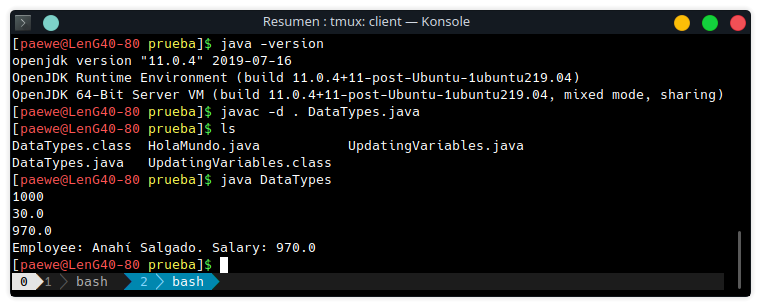
\includegraphics[scale=0.75]{./Pictures/039_DataTypes.png}
\end{figure}

\textbf{Nota:} Para este ejercicio se usó \textbf{Java 11 con OpenJDK}


%% Clase 16
\section{Operadores de Asignación, incremento y Decremento}%
\textbf{Operadores de asignación}:\\
\begin{itemize}
  \item \textbf{$+=$}: $a += b$ es equivalente a $a = a + b$
  \item \textbf{$-=$}: $a -= b$ es equivalente a $a = a - b$
  \item \textbf{$*=$}: $a *= b$ es equivalente a $a = a * b$
  \item \textbf{$/=$}: $a /= b$ es equivalente a $a = a / b$
  \item \textbf{$\%=$}: $a \%= b$ es equivalente a $a = a \% b$
\end{itemize}

\textbf{Operadores de incremento}:\\
\begin{itemize}
  \item \textbf{$++$}: $i++$ es equivalente a $i = i + 1$
  \item \textbf{$--$}: $i--$ es equivalente a $i = i - 1$
\end{itemize}

Podemos usar estos operadores de forma prefija $(++1)$ o postfija $(i++)$. La
diferencia está en qué operación se ejecutará primero:

\begin{minted}{java}
  public class IncrementDecrement {
      public static void main(String[] args) {
          int lives = 5;
          lives = lives - 1;
          System.out.println(lives);  // 4

          lives--;                    // decremento
          System.out.println(lives);  // 3

          lives++;                    // incremento
          System.out.println(lives);  // 4

          // Prefija
          // Gana un regalo por ganar una vida
          int gift = 100 + lives++;   // postfijo
          System.out.println(gift);   // 104
          System.out.println(lives);  // 5

          gift = 100 + ++lives;       // prefija
          System.out.println(gift);   // 106
          System.out.println(lives);  // 6
      }
  }
\end{minted}

\begin{figure}[h!]
  \centering
  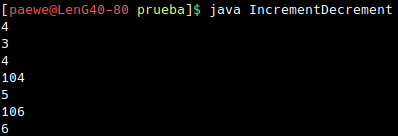
\includegraphics[scale=0.75]{./Pictures/040_Increment_Decrement.png}
\end{figure}


%% Clase 17
\section{Operaciones matemáticas}%
\texttt{Math} es una clase de Java que nos ayuda a ejecutar diferentes
operaciones matemáticas:

\begin{minted}{java}
  public class MathematicOperations {
      public static void main(String[] args) {
          double x = 2.1;
          double y = 3;

          // Devuelve un entero hacia arriba
          System.out.println(Math.ceil(x));

          // Devuelve un entero hacia abajo
          System.out.println(Math.floor(x));

          // Devuelve un número elevado a otro número
          System.out.println(Math.pow(x,y));

          // Devuelve el número mayor
          System.out.println(Math.max(x,y));

          // Devuelve la raíz cuadrada
          System.out.println(Math.sqrt(y));

          // Area de un círculo
          // pi*r2
          System.out.println(Math.PI * Math.pow(y,2));

          // Area de una esfera
          // 4*pi*r2
          System.out.println(4*Math.PI*Math.pow(y,2));

          // Volumen de una esfera
          // (4/3)*pi*r3
          System.out.println((4/3) * Math.PI * Math.pow(y,3));
      }
  }
\end{minted}

Una de las ventajas de usar un IDE como \textbf{IntelliJ IDEA} es que cuando se
necesita invocar un procedimiento como en este caso, se hace de una manera
mucho más práctica:

\begin{figure}[h!]
  \centering
  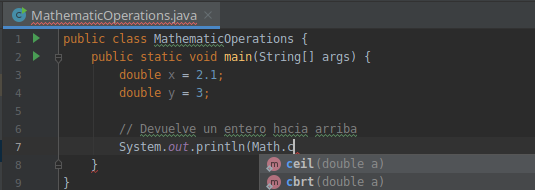
\includegraphics[scale=0.75]{./Pictures/041_MathematicOperations.png}
\end{figure}

\begin{figure}[h!]
  \centering
  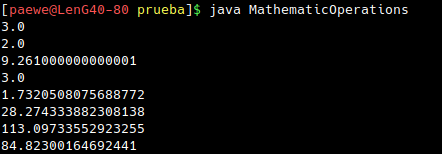
\includegraphics[scale=0.75]{./Pictures/042_MathematicOperations.png}
\end{figure}


%% Clase 18
\section{Cast en variables: Estimación y Exactitud}%
En la programación hay situaciones donde necesitamos cambiar el tipo de dato de
nuestras variables, esto lo conocemos como \textbf{Cast}. \textbf{Estimación}.

\begin{minted}{java}
  public class Casting {
      public static void main(String[] args) {
          // En un año ubicar 30 perritos
          // Cuantos perritos ubiqué al mes

          double monthlyDogs = 30.0/12.0;
          System.out.println(monthlyDogs);

          // ESTIMACION
          int estimatedMonthlyDogs = (int) monthlyDogs;
          System.out.println(estimatedMonthlyDogs);

          // Exactitud
          int a = 30;
          int b = 12;
          System.out.println((double)a/b);
      }
  }
\end{minted}

\begin{figure}[h!]
  \centering
  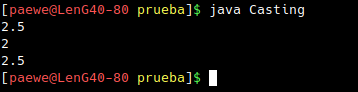
\includegraphics[scale=0.75]{./Pictures/043_Casting.png}
\end{figure}


%% Clase 19
\section{Casteo entre tipo e datos}%
Java nos ayuda a realizar casteo automático de los tipos de datos más chicos a
otros más grandes. Sin embargo, en algunos casos vamos a necesitar realizar un
cast manualmente, así como aprendimos en la clase anterior (\texttt{(dataType)
variableOperacion}).\\

Por ejemplo supongamos que declaramos dos variables a y b de tipo int y una
variable c de tipo double que es igual a la división de las primeras dos
variables.\\

En este caso, aunque definimos que el tipo de dato de c es double, Java
automáticamente convertirá el resultado de la división a tipo int, ya que este
es el tipo de datos de las dos variables que dividimos, pero seguirá respetando
que la variable c es de tipo double y añadirá un decimal al final (.0).

\begin{figure}[h!]
  \centering
  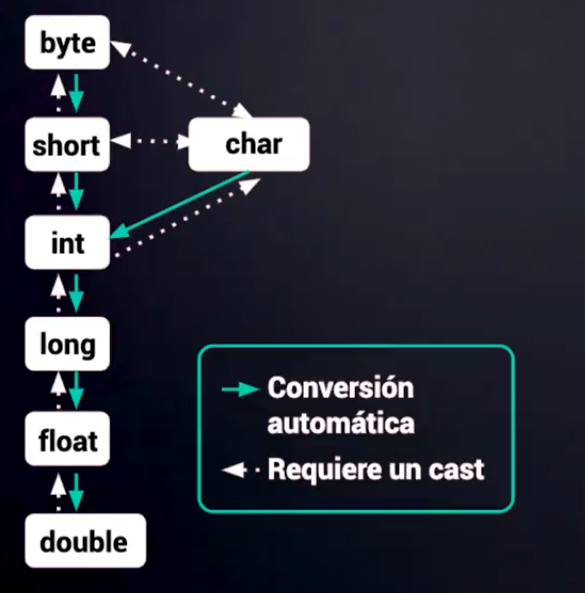
\includegraphics[scale=0.75]{./Pictures/003_conversiones.png}
\end{figure}


Esto significa que muchas de nuestras operaciones pueden verse afectadas. Por
ejemplo:

\begin{minted}{java}
  public class Casting {
      public static void main(String[] args) {
          // En un año ubicar 30 perritos
          // Cuantos perritos ubiqué al mes

          double monthlyDogs = 30.0/12.0;
          System.out.println(monthlyDogs);

          // ESTIMACION
          int estimatedMonthlyDogs = (int) monthlyDogs;
          System.out.println(estimatedMonthlyDogs);

          // Exactitud
          int a = 30;
          int b = 12;
          System.out.println((double)a/b);

          double c = (double) a/b;
          System.out.println(c);

          char n = '1';
          int nI = n;
          System.out.println(nI);

          short nS = (short) n;
          System.out.println(nS);
      }
  }
\end{minted}

Si en la variable c no se le asigna la division de los enteros a y b con cast
double, entonces guardará el resultado de la división entera casteado a double,
es decir 2.0. Pero si queremos exactitud entonces deberemos castear
explicitamente con double delante de la división.

\begin{figure}[h!]
  \centering
  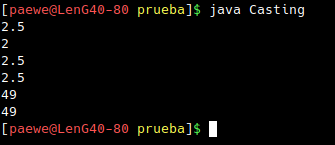
\includegraphics[scale=0.75]{./Pictures/044_Casting.png}
\end{figure}


\newpage
%% Clase 20
\section{Archivos .JAR}%
Los archivos JAR (Java Archive) son archivos de Java con el código compilado de
los archivos \texttt{.class} y comprimido con el formato ZIP para que adelante
sean interpretados y ejecutados por la máquina viertual de Java (JVM).\\

Para generar estos archivos podemos entrar a \texttt{File > Project Structure >
Artifacts} y seleccionar la opción de \texttt{JAR > From modules with
dependencies}.

\begin{figure}[h!]
  \centering
  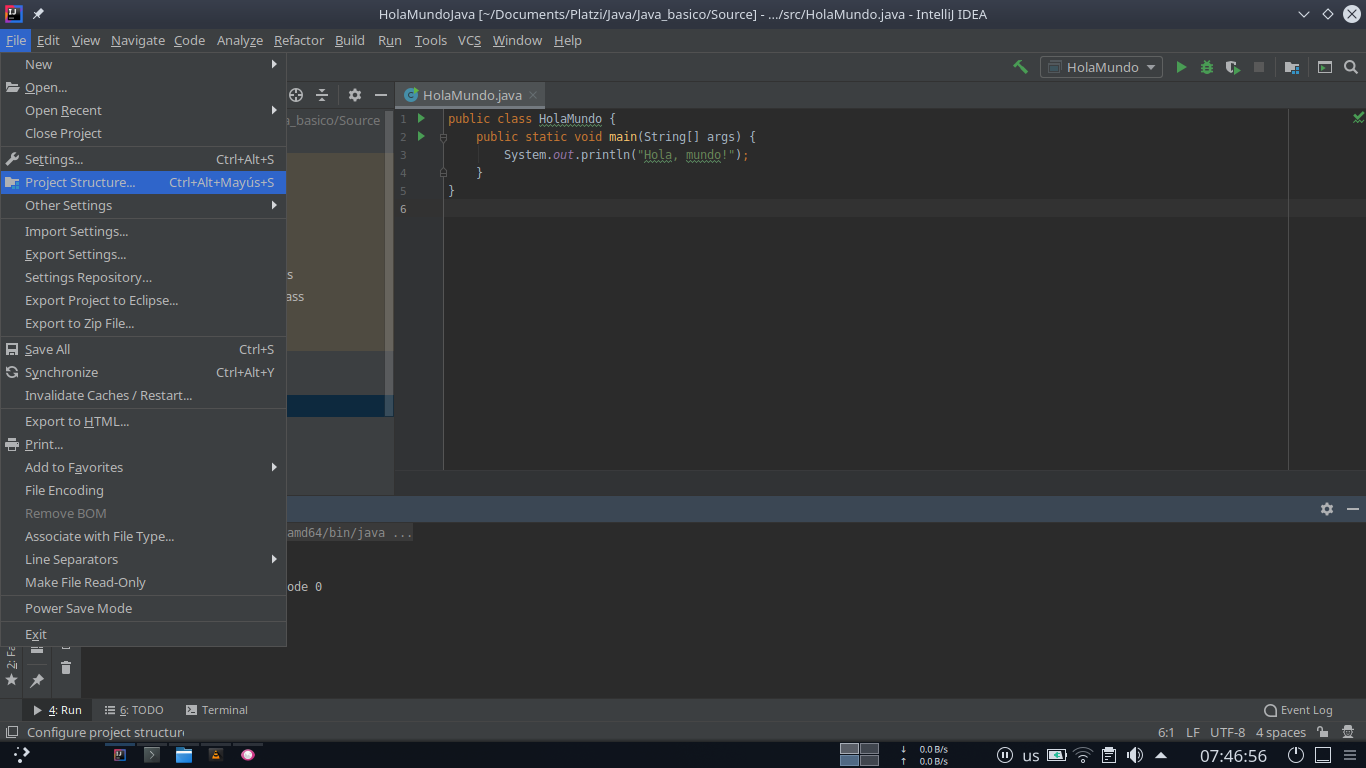
\includegraphics[scale=0.45]{./Pictures/004_jar.png}
\end{figure}

\begin{figure}[h!]
  \centering
  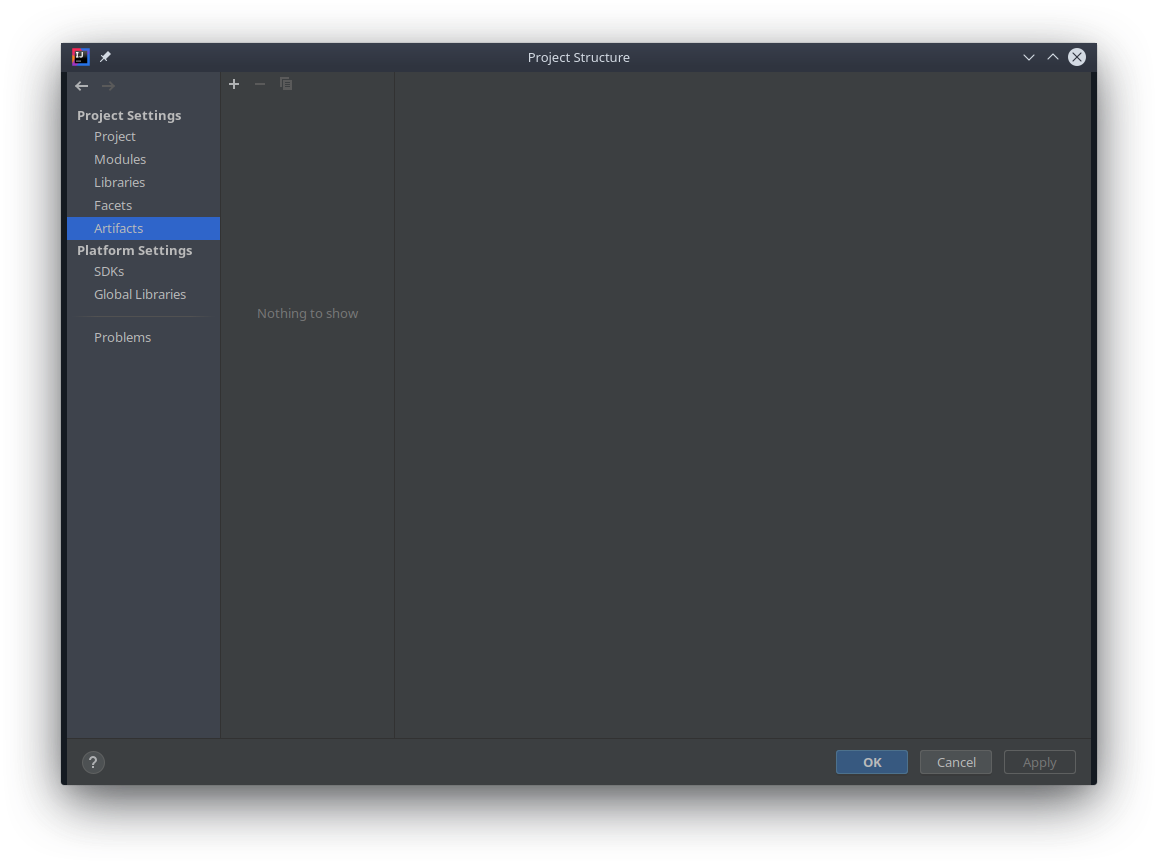
\includegraphics[scale=0.55]{./Pictures/005_jar.png}
\end{figure}

\newpage

\begin{figure}[h!]
  \centering
  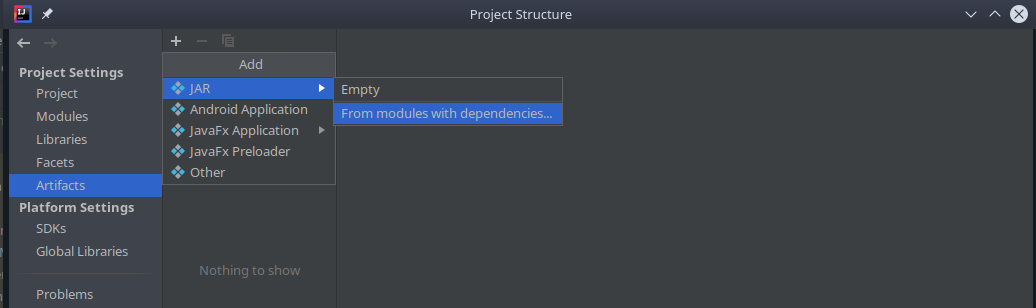
\includegraphics[scale=0.55]{./Pictures/006_jar.png}
\end{figure}

\begin{figure}[h!]
  \centering
  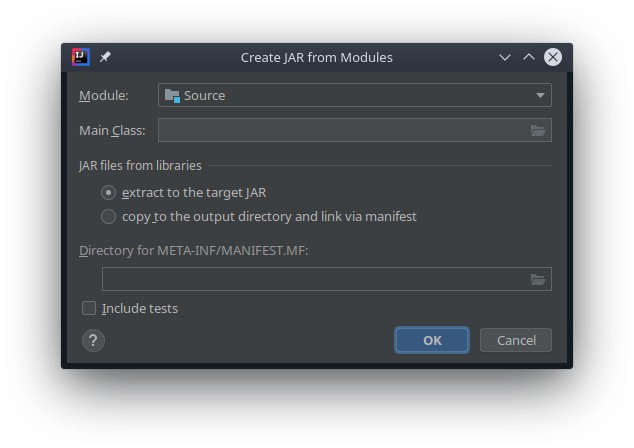
\includegraphics[scale=0.65]{./Pictures/007_jar.png}
\end{figure}

\begin{figure}[h!]
  \centering
  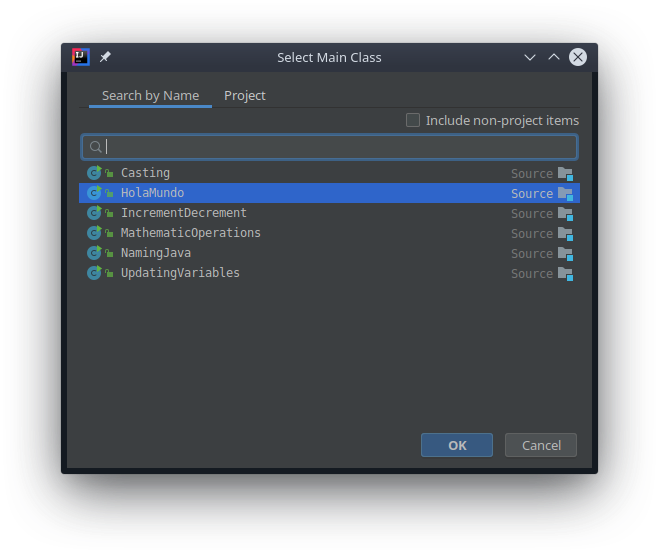
\includegraphics[scale=0.60]{./Pictures/008_jar.png}
\end{figure}

\newpage

\begin{figure}[h!]
  \centering
  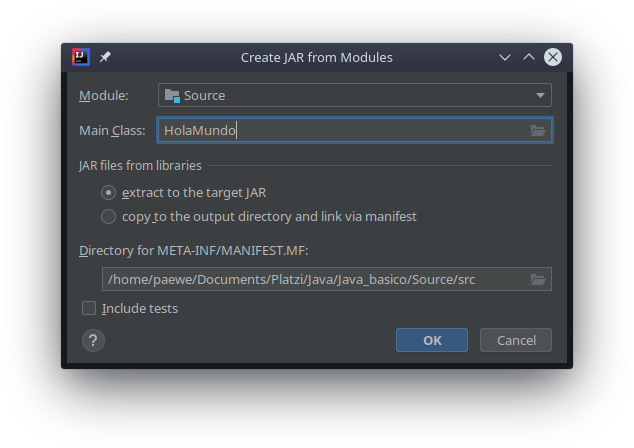
\includegraphics[scale=0.60]{./Pictures/009.png}
\end{figure}

Luego de esto podemos compilar nuestro proyecto desde \texttt{Build > Build
Artifacts > Build} los archivos ejecutables se almacenarán en la carpeta
\texttt{out/artifacts/}.

\begin{figure}[h!]
  \centering
  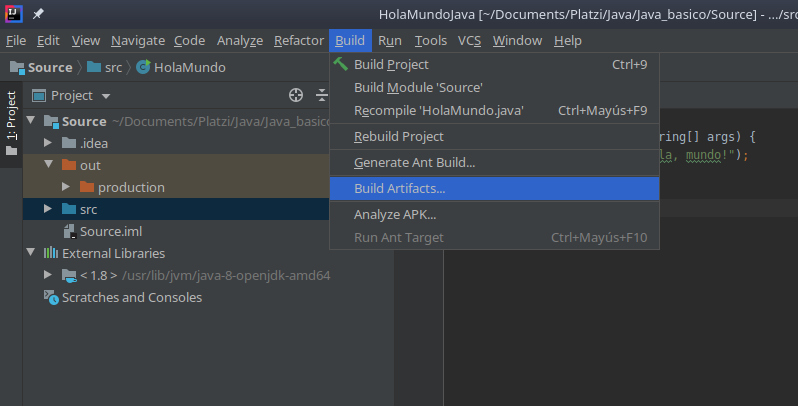
\includegraphics[scale=0.65]{./Pictures/010_jar.png}
\end{figure}

\begin{figure}[h!]
  \centering
  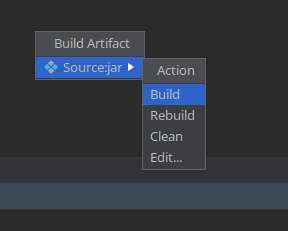
\includegraphics[scale=0.65]{./Pictures/011_jar.png}
\end{figure}

\begin{figure}[h!]
  \centering
  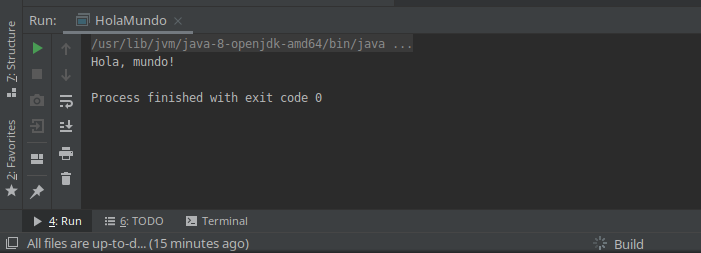
\includegraphics[scale=0.75]{./Pictures/012_jar.png}
\end{figure}

\newpage

\begin{figure}[h!]
  \centering
  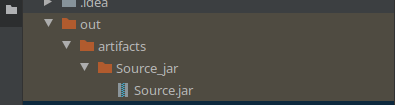
\includegraphics[scale=0.75]{./Pictures/013_jar.png}
\end{figure}

%\begin{figure}[h!]
%  \centering
%  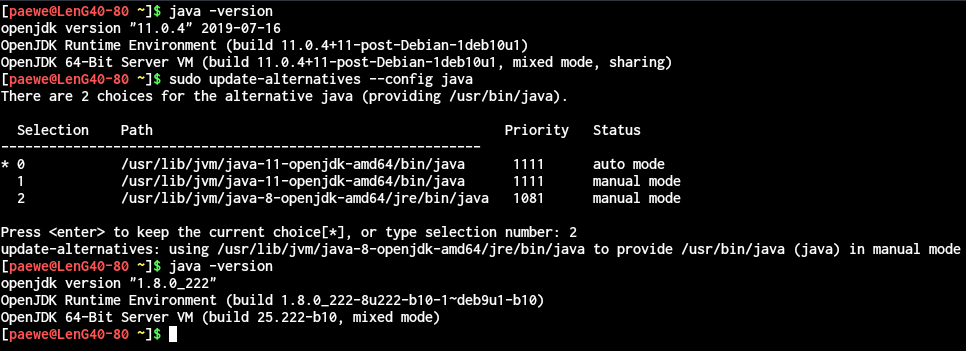
\includegraphics[scale=0.70]{./Pictures/014.png}
%\end{figure}

\begin{figure}[h!]
  \centering
  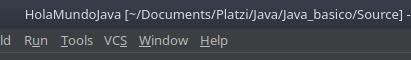
\includegraphics[scale=0.75]{./Pictures/015_jar.png}
\end{figure}

\begin{figure}[h!]
  \centering
  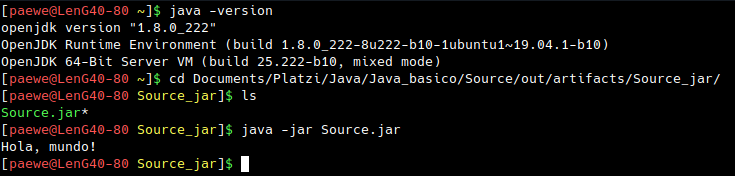
\includegraphics[scale=0.75]{./Pictures/016_jar.png}
\end{figure}

Hacemos lo mismo para el proyecto creado usando Java 11.

\begin{figure}[h!]
  \centering
  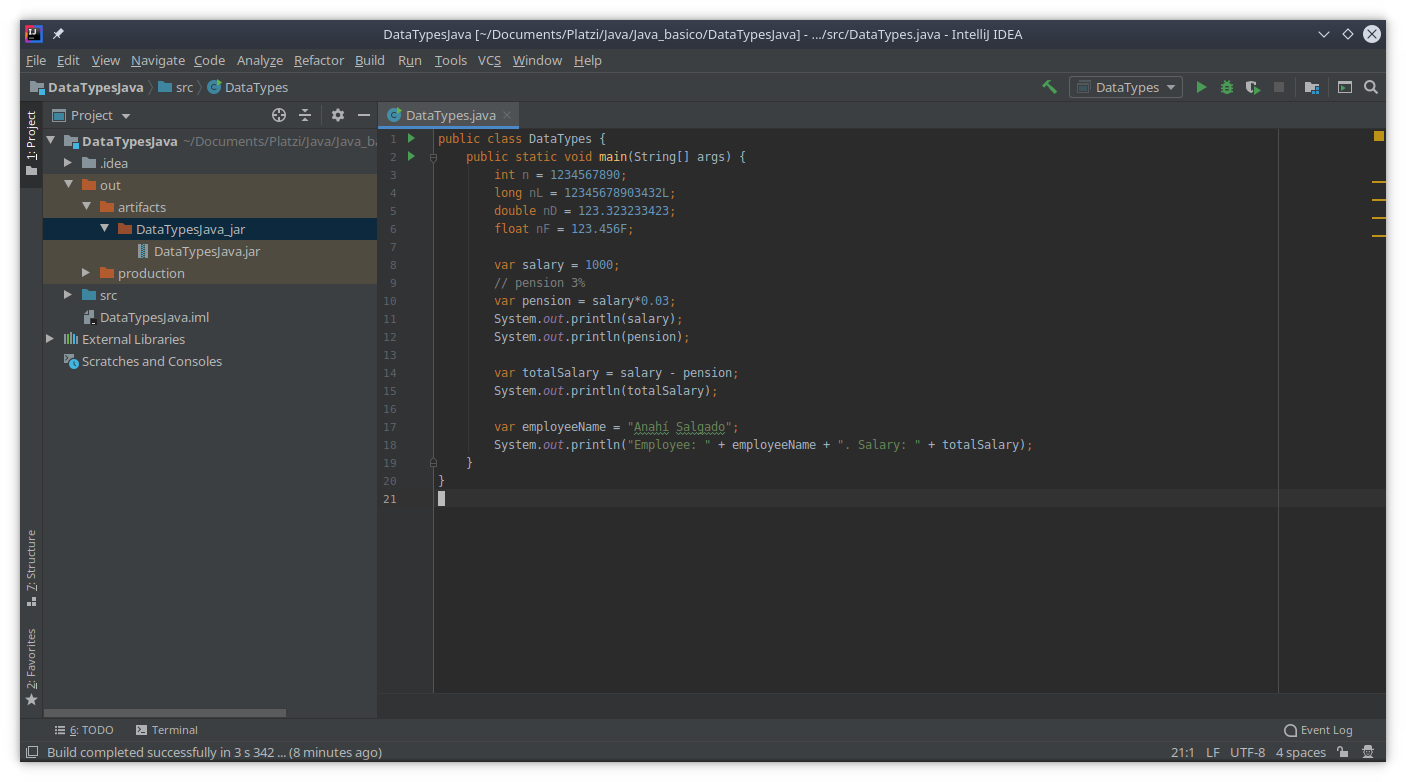
\includegraphics[scale=0.45]{./Pictures/017_jar.png}
\end{figure}

\begin{figure}[h!]
  \centering
  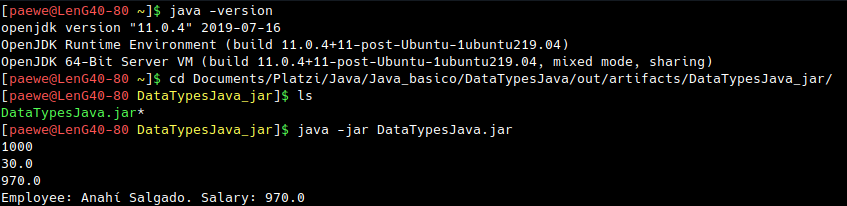
\includegraphics[scale=0.75]{./Pictures/018_jar.png}
\end{figure}

\newpage

%% Clase 22
\section{Sentencia if}%
Los condicionales son la forma en que las computadoras toman decisiones,
evaluarán si la condición para ejecutar una parte del código se cumple. Si el
resultado de la operación es verdadero ejecutarán esta parte del código, en
caso de que no, seguirán con las siguientes instrucciones.\\

La forma de programar condicionales es usando la sentencia IF (hay más, pero
las veremos más adelante). En el siguiente ejemplo vamos a guardar algunas
instrucciones dentro del condicional if, Java solo ejecutará esta parte del
código si se cumple la condición, en este caso, que la variable
\texttt{isBlueToothEnabled} sea igual a true:


\begin{minted}{java}
  public class IfStatement {
      public static void main(String[] args) {
          boolean isBluetoothEnabled = true;
          int fileSend = 3;

          if (isBluetoothEnabled) {
              // Send file
              fileSend++;
              System.out.println("Archivo Enviado");
          }
      }
  }
\end{minted}

\begin{figure}[h!]
  \centering
  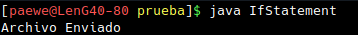
\includegraphics[scale=0.75]{./Pictures/045_if_statement.png}
\end{figure}


%% Clase 23
\section{Alcance de las variables y Sentencia ELSE}%
Mientras más crecen nuestros programas, más lógica, complejidad y niveles
añadimos. Estos niveles son el alcance que tienen nuestras variables, es decir,
los lugares donde pueden ejecutarse o no.\\

Estos niveles (en parte) son representados por las llaves ($\{ \cdots \}$) que
envuelven nuestro código, estaremos más niveles dentro y el alcance de las
variables que definimos será un poco más limitado.\\

Solo podemos usar una variable si la definimos antes, en el mismo nivel o
alguno anterior. Pero si declaramos una variable en un nivel posterior al resto
de nuestro código, no podremos modificarla a menos que el código esté en su
mismo nivel.\\

Por ejemplo:\\

\begin{minted}{java}
  public class IfStatement {
      public static void main(String[] args) {
          boolean isBluetoothEnable = true;
          int fileSend = 3;

          if (isBluetoothEnable) {
              // Send file
              fileSend++;
              System.out.println("Archivo Enviado");
              int i = 0;
              i++;
          } else {
              System.out.println("Por favor, enciende tu bluetooth,
                                  para iniciar la transferencia");
          }

          System.out.println(isBluetoothEnable);
          System.out.println(fileSend);
          // System.out.println(i);  Variable i no está al alcance
      }
  }
\end{minted}

\begin{figure}[h!]
  \centering
  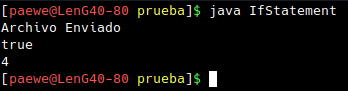
\includegraphics[scale=0.75]{./Pictures/046_alcance.png}
\end{figure}

La sentencia \texttt{ELSE} es todo lo contrario a la sentencia \texttt{IF}: en
vez de ejecutar una parte del código si la condición es verdadera, solo lo hará
si la condición \texttt{NO} se cumple.


%% Clase 24
\section{Operadores Lógicos y Expresiones booleanas}%
Nuestros condicionales no solo pueden evaluar variables booleanas, también
pueden evaluar si el resultado de una ooperación es verdadero o falso. Para
esto debemos usar los operadores lógicos:\\

\textbf{Operadores de equidad}\\
\begin{figure}[h!]
  \centering
  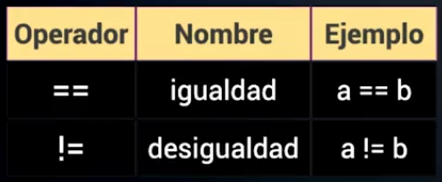
\includegraphics[scale=0.75]{./Pictures/019_equidad.png}
\end{figure}

\textbf{Operadores de relación}\\
\begin{figure}[h!]
  \centering
  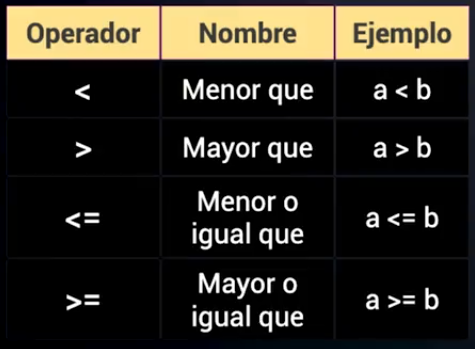
\includegraphics[scale=0.75]{./Pictures/020_relacionales.png}
\end{figure}

\newpage

\textbf{Operadores lógicos}\\
\begin{figure}[h!]
  \centering
  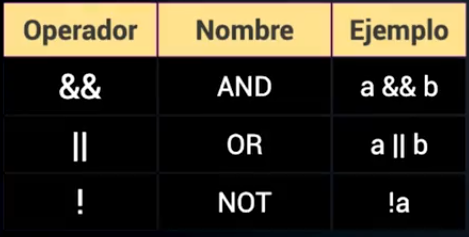
\includegraphics[scale=0.75]{./Pictures/021_logicos.png}
\end{figure}

\begin{figure}[h!]
  \centering
  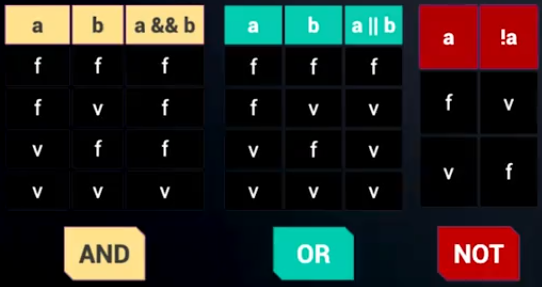
\includegraphics[scale=0.75]{./Pictures/022_logicos.png}
\end{figure}


\begin{minted}{java}
  public class LogicOperations {
      public static void main(String[] args) {
          int a = 8;
          int b = 5;

          // Operadores de equidad
          System.out.println("a es igual a b? -> " + (a == b));
          System.out.println("a es diferente a b? -> " + (a != b));

          // Operadores relacionales
          System.out.println("a es mayor a b? -> " + (a > b));
          System.out.println("a es menor a b? -> " + (a < b));
          System.out.println("a es mayor o igual a b? -> " + (a >= b));
          System.out.println("a es menor o igual a b? -> " + (a <= b));

          if (a == b) {
              System.out.println("a es igual a b");
          } else if (a != b) {
              System.out.println("a es diferente de b");
          }

          if (a > b) {
              System.out.println("a es mayor a b");
          } else if (a < b) {
              System.out.println("a es menor a b");
          } else if (a >= b) {
              System.out.println("a es mayor o igual a b");
          } else if (a <= b) {
              System.out.println("a es menor o igual a b");
          }
      }
  }
\end{minted}

\begin{figure}[h!]
  \centering
  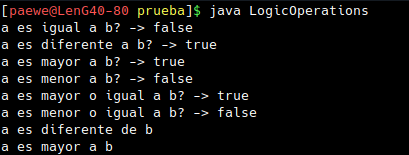
\includegraphics[scale=0.75]{./Pictures/047_logic.png}
\end{figure}


%% Clase 25
\section{Sentencia Switch}%
La sentencia Switch nos ayuda a tomar decisiones con base en una o más
condicionales, pero funciona un poco diferente.

\begin{figure}[h!]
  \centering
  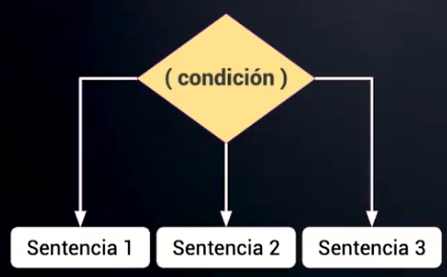
\includegraphics[scale=0.75]{./Pictures/023_switch.png}
\end{figure}


\begin{minted}{java}
  public class SwitchStatement {
      public static void main(String[] args) {
          String colorModeSelected = "Dark";

          switch (colorModeSelected) {
              case "Light":
                  System.out.println("Seleccionaste Light Mode");
                  break;
              case "Night":
                  System.out.println("Seleccionaste Night Mode");
                  break;
              case "Blue Dark":
                  System.out.println("Seleccionaste Blue Dark Mode");
                  break;
              case "Dark":
                  System.out.println("Seleccionaste Dark Mode");
                  break;
              default:
                  System.out.println("Selecciona una opción válida");
          }
      }
  }
\end{minted}

\begin{figure}[h!]
  \centering
  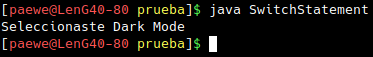
\includegraphics[scale=0.75]{./Pictures/048_switch.png}
\end{figure}


%% Clase 26
\section{¿Para qué sirven las funciones?}%

\begin{figure}[h!]
  \centering
  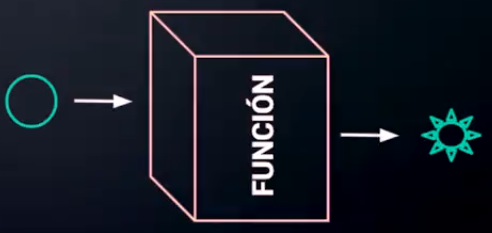
\includegraphics[scale=0.75]{./Pictures/024_funcion.png}
\end{figure}

Las funciones nos ayudan a ejecutar código que dependiendo de las opciones que
le enviemos, transformará y devolverá un cierto resultado. Gracias a las
funciones podemos organizar, modularizar, reutilizar y evitar repetidos en
nuestro código.\\

\begin{figure}[h!]
  \centering
  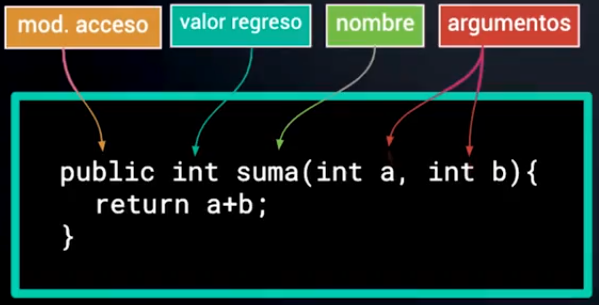
\includegraphics[scale=0.75]{./Pictures/025_funcion.png}
\end{figure}

Todas nuestras funciones deben tener un nombre. Opcionalmente, pueden recibir
argumentos y devolver un resultado. También debemos especificar el tipo de dato
de nuestros argumentos y el resultado final de nuestra función.\\

Al llamar una función:

\begin{figure}[h!]
  \centering
  \includegraphics[scale=0.75]{./Pictures/026_funcion.png}
\end{figure}

\newpage

%% Clase 27
\section{Implementa funciones en Java}%
Cuando se tiene que repetir mucho una instrucción de código es conveniente usar funciones.

\begin{minted}{java}
  public class Funciones {
      public static void main(String[] args) {
          double y = 3;
          double areaCirculo, areaEsfera, volumenEsfera;

          // Área de un círculo
          // pi*r2
          circleArea(y);

          // Área de una esfera
          // 4*pi*r2
          sphereArea(y);

          // Volumen de una esfera
          // (4/3)*pi*r3
          sphereVolumen(y);

          System.out.println("Area circulo: " + areaCirculo + ". Area esfera: " +
                                areaEsfera + ". Volumen esfera: " + volumenEsfera);
          System.out.println("PESOS A DOLARES: " + converToDolar(1000, "COP"));
      }

      public static double circleArea(double r) {
          return 2*Math.PI*Math.pow(r,2);
      }

      public static double sphereArea(double r) {
          return 4*Math.PI*Math.pow(r,2);
      }

      public static double sphereVolumen(double r) {
          return (4/3)*Math.PI*Math.pow(r,3);
      }

      public static double converToDolar(double quantity, String currency) {
          // MXN COP
          switch (currency) {
              case "MXN":
                  quantity = quantity*0.052;
                  break;
              case "COP":
                  quantity = quantity*0.00031;
                  break;
          }
          return quantity;
      }
  }
\end{minted}

\newpage

\begin{figure}[h!]
  \centering
  \includegraphics[scale=0.75]{./Pictures/049_funciones.png}
\end{figure}


%% Clase 28
\section{Java Docs}%
Los Java Docs son una herramienta usada por muchas otras herramientas y
aplicaciones porque nos ayuda a documentar todo nuestro código usando
comentarios. Además, nos permite visualizar la documentación en formato HTML.

Por ejemplo veamos la documentación que usa
\href{https://developer.android.com/reference/android/support/v4/media/MediaBrowserCompat}{Android}
con JavaDoc:

\begin{figure}[h!]
  \centering
  \includegraphics[scale=0.5]{./Pictures/050_javadocs_android.png}
\end{figure}

También \href{https://docs.spring.io/spring-boot/docs/2.2.0.M6/api/}{Spring},
que es un framework de java usa javadocs para su documentación.

\begin{figure}[h!]
  \centering
  \includegraphics[scale=0.5]{./Pictures/051_javadocs_spring.png}
\end{figure}

Y todo esto se logra con la magia de los comentarios:
\begin{minted}{java}
  // Comentarios de una línea
  /* Comentarios en multiples líneas */
  /** Comentarios para Javadocs */
\end{minted}

%% Clase 29
\section{Javadoc en Funciones }%
Vamos a documentar la función \texttt{convertToDolar}. Recuerda que esta
función devuelve un número \texttt{double} y recibe dos argumentos:
\texttt{quantity} (de tipo \texttt{double} y \texttt{currency} (de tipo
\texttt{String}):


\begin{minted}{java}
  public class Funciones {
      public static void main(String[] args) {
          double y = 3;

          // Área de un círculo
          // pi*r2
          circleArea(y);

          // Área de una esfera
          // 4*pi*r2
          sphereArea(y);

          // Volumen de una esfera
          // (4/3)*pi*r3
          sphereVolumen(y);

          System.out.println("PESOS A DOLARES: " + converToDolar(1000, "COP"));
      }

      public static double circleArea(double r) {
          return 2*Math.PI*Math.pow(r,2);
      }

      public static double sphereArea(double r) {
          return 4*Math.PI*Math.pow(r,2);
      }

      public static double sphereVolumen(double r) {
          return (4/3)*Math.PI*Math.pow(r,3);
      }

      /**
      * Descripción: Función que especificando su moneda convierte una cantidad de dinero a dólares
      * @param quantity Cantidad de dinero
      * @param currency Tipo de Moneda: Solo acepta MXN o COP
      * @return quantity Devuelve la cantidad actualizada en Dolares
      */
      public static double converToDolar(double quantity, String currency) {
          // MXN COP
          switch (currency) {
              case "MXN":
                  quantity = quantity*0.052;
                  break;
              case "COP":
                  quantity = quantity*0.00031;
                  break;
          }
          return quantity;
      }
  }
\end{minted}

%% Clase 30
\section{Tags Java Docs}%

\begin{figure}[h!]
  \centering
  \includegraphics[scale=0.65]{./Pictures/028_javadocs_flags.jpg}
\end{figure}


%% Clase 31
\section{Bucle do While}%
Los bucles (ciclos) nos ayudan a ejecutar una parte de nuestro código una
cantidad de veces hasta que se cumpla alguna condición y podamos continuar con
la ejecución de nuestro código.\\

Existen diferentes bucles. Por ejemplo, el bucle \texttt{while}:

\begin{figure}[h!]
  \centering
  \includegraphics[scale=0.75]{./Pictures/028_while.png}
\end{figure}

Veamos un ejemplo para Do while:

\begin{minted}{java}
  import java.util.Scanner;

  public class DoWhileLoop {
      public static void main(String[] args) {
          int response = 0;
          do {
              System.out.println("Selecciona el número de la opción deseada");
              System.out.println("1. Movies");
              System.out.println("2. Series");
              System.out.println("0. Salir");

              Scanner sc = new Scanner(System.in);
              response = Integer.valueOf(sc.nextLine());

              switch (response) {
                  case 0:
                      System.out.println("Gracias por visitarnos");
                      break;
                  case 1:
                      System.out.println("Movies");
                      break;
                  case 2:
                      System.out.println("Series");
                      break;
                  default:
                      System.out.println("Selecciona una opción correcta");
              }
          } while (response != 0);
          System.out.println("Se terminó el programa");
      }
  }
\end{minted}


%% Clase 32
\section{Operador Ternario y Bucle While}%
Vamos a crear el algoritmo con la lógica necesaria para encender una lámpara,
emitir un mensaje y detener las luces en algún momento.\\

El Bucle While nos ayuda a ejecutar una parte del código mientras una condición
se cumpla. Recuerda tener mucho cuidado y asegurarte de que la condición del
ciclo While cambie en algún momento, de otra forma, el ciclo no se detendrá
nunca y sobrecargarás tu programa.

\begin{minted}{java}
  public class WhileLoop {
      static boolean isTurnOnLight = false;

      public static void main(String[] args) {
          turnOnOffLight();

          int i = 1;
          while (isTurnOnLight && i<=10) {
              printSOS();
              i++;
          }
      }

      public static void printSOS() {
          System.out.println(". . . _ _ _ . . .");
      }

      public static boolean turnOnOffLight() {
          isTurnOnLight = (isTurnOnLight)?false:true;     // Operador terniario
      //    if (isTurnOnLight) {
      //        isTurnOnLight = false;
      //    } else {
      //        isTurOnLight = true;
      //    }
          return isTurnOnLight;
      }
  }
\end{minted}

%% Clase 33
\section{Bucle For}%
El Ciclo For también nos ayuda a ejecutar una parte de nuestro código las veces
que sean necesarias para que se cumplan una condición. de hecho, el ciclo
\texttt{FOR} nos da muchas ayudas para lograr este resultado de la forma más
fácil posible:\\

\begin{figure}[h!]
  \centering
  \includegraphics[scale=0.75]{./Pictures/029_for.png}
\end{figure}

\begin{minted}{java}
  public class ForLoop {

      static boolean isTurnOnLight = false;

      public static void main(String[] args) {
          turnOnOffLight();

          for (int i = 1; i <= 10 ; i++) {
              printSOS();
          }
      }

      public static void printSOS() {
          System.out.println(". . . _ _ _ . . .");
      }

      public static boolean turnOnOffLight() {
          isTurnOnLight = (isTurnOnLight)?false:true;     // Operador terniario
          return isTurnOnLight;
      }
  }
\end{minted}


%% Clase 34
\section{Break, Continue y Return}%
Antes de pasar a uno de nuestros temas más importantes del curso es importante
que sepas todas las opciones que tienes para detener ciclos y así seguir
controlando el flujo de tus programas.

\textbf{Break}\\
En Java esta sentencia la verás en dos situaciones específicamente:
\begin{enumerate}
  \item En un \textbf{Switch}: en esta situación break hace que el flujo del
    switch no continúe ejecutándose a la siguiente comparación, esto con el
    objetivo de que solo se cumpla una sola condición:

  \begin{minted}{ipython3}
    switch (colorModelSelected) {
      case "Light":
        System.out.println("Seleccionaste Light Mode");
        break;
      case "Night":
        System.out.println("Seleccionaste Night Mode");
        break;
      case "Blue Dark":
        System.out.println("Seleccionaste Blue Dark Mode");
        break;
    }
  \end{minted}

  \item Para salir de un \textbf{bucle}: Como acabamos de ver un break es capaz
    de detener el flujo en el código, en este caso detendremos el ciclo como
    tal terminándolo y haciendo que saltemos a la siguiente instrucción después
    del ciclo.
\end{enumerate}

\textbf{Continue}\\
Continue en cierto modo también nos va a servir para detener un ciclo pero en
lugar de terminarlo como en el caso de break, este volverá directo a la
condición.\\

\textbf{Return}\\
Aunque en algunos lenguajes esta sentencia sirve como un tipo goto, dónde se
rompe el flujo del programa la mejor forma de usarlo en Java es en
\textbf{Funciones}, cuando lo usamos aquí siempre viene acompañado de un valor,
el cuál indica el dato que se estará devolviendo en la función.


%% Clase 35
\section{Arrays}%
Los arreglos o arrays son objetos en los que podemos guardar más de una
variable, una lista de elementos. Los arrays son de una sola dimensión, pero si
guardamos arrays dentro de otros arrays podemos obtener arrays
multidimensionales.\\

Los arrays se definen en código de las siguientes maneras:

\begin{minted}{java}
  // 1. Definir el nombree de la variable y el tipo de dato.
  TipoDato[] nombreVariable;
  TipoDato el tamaño del array, la cantidad de elemntos que podemos
  TipoDato[] nombreVariable;
  TipoDato nombreVariable[];

  // 2. Definir el tamaño del array, la cantidad de elementos
  // que podemos guardar en el carry.
  TipodDato[] = new TipoDatos[capacidad];

  // Array de dos dimensiones
  TipoDato[][] cites = new String[númeroFilas][númeroColumnas];
\end{minted}

Ya que los arrays pueden guardar múltiples elementos, la conveción es escribir
los nombres de las variables en plural.

%% Clase 36
\section{Declarando Arreglos}%

\begin{minted}{java}
  public class Arrays {
      public static void main(String[] args) {
          String[] androidVersions = new String[17];
          String days[] = new String [7];

          String[][] cities = new String[4][2]; // 4*2 = 8
          /*
          * +--------------------------+
          * | Country    | City        |
          * ----------------------------
          * | México     | CDMX        |
          * | México     | Guadalajara |
          * | Colombia   | Bogotá      |
          * | Colombia   | Medellín    |
          * +--------------------------+
          **/

          int[][][] numbers = new int[2][2][2];
          int[][][][] numbers4 = new int[2][2][2][2];
      }
  }
\end{minted}


%% Clase 37
\section{Índices y búsqueda de elementos en Arrays}%
Los índices son variables simples que nos ayudan a indentificar las posicioness
en un arreglo. Estas variables siempre guardan números, comienzan en 0 e
incrementan de arriba a abajo y de izquierda a derecha a medida que guardamos
más elementos en nuestros arrays.\\

Para guardar un valor en alguna posición de nuestro array solo debemos usar el
índice de la siguiente forma:

\begin{minted}{java}
  nombreVariable[indice] = valor;
\end{minted}

Recuerda que puedes aprender mucho más sobre estructura de datos en el
\textbf{Curso Básico de Algoritmos}.

\begin{minted}{java}
  public class Arrays {
      public static void main(String[] args) {
          String[] androidVersions = new String[17];
          String days[] = new String [7];

          String[][] cities = new String[4][2]; // 4*2 = 8
          /*
          * +--------------------------+
          * | Country    | City        |
          * ----------------------------
          * | México     | CDMX        |
          * | México     | Guadalajara |
          * | Colombia   | Bogotá      |
          * | Colombia   | Medellín    |
          * +--------------------------+
          **/

          int[][][] numbers = new int[2][2][2];
          int[][][][] numbers4 = new int[2][2][2][2];

          androidVersions[0] = "Apple Pie";
          androidVersions[1] = "Bannana Bread";
          androidVersions[2] = "Cupcake";
          androidVersions[3] = "Donut";

          System.out.println(androidVersions[0]);
          System.out.println(androidVersions[1]);
          System.out.println(androidVersions[2]);
          System.out.println(androidVersions[3]);

          System.out.println();
          System.out.println();

          cities[0][0] = "Colombia";
          cities[0][1] = "Medellín";
          cities[1][0] = "colombia";
          cities[1][1] = "Bogotá";
          cities[2][0] = "México";
          cities[2][1] = "Guadalajara";
          cities[3][0] = "México";
          cities[3][1] = "CDMX";

          System.out.println(cities[0][0]);
          System.out.println(cities[0][1]);
          System.out.println(cities[1][0]);
          System.out.println(cities[1][1]);
          System.out.println(cities[2][0]);
          System.out.println(cities[2][1]);
          System.out.println(cities[3][0]);
          System.out.println(cities[3][1]);

          String[][][][] animals =  new String[2][3][2][2];
          animals[1][0][0][1] = "Monkey";

          System.out.println();
          System.out.println();
          System.out.println(animals[1][0][0][1]);

      }
  }
\end{minted}


%% Clase 38
\section{Ciclos For anidados}%
Los ciclos \texttt{FOR} nos ayudan a ejecutar una parte de nuestro código todas
las veces que sean necesarias hasta que una condición se cumpla por ejemplo,
que un número supere o iguale cierta cantidad.\\

Eso es exactamente lo que necesitamos para trabajar con índices. En vez de
escribir todos los números a mano, vamos a utilizar un ciclo para imprimir el
valor de cada posición de nuestros arreglos, incluso si estos son
multidimensionales.\\






















\vspace{2cm}
\LARGE\textit{RuneCode}


\end{document}

